% arara: makeindex

% Template for IEEE papers
%% bare_conf.tex
%% V1.4b
%% 2015/08/26
%% by Michael Shell
%% See:
%% http://www.michaelshell.org/
%% for current contact information.
%%
%% This is a skeleton file demonstrating the use of IEEEtran.cls
%% (requires IEEEtran.cls version 1.8b or later) with an IEEE
%% conference paper.
%%
%% Support sites:
%% http://www.michaelshell.org/tex/ieeetran/
%% http://www.ctan.org/pkg/ieeetran
%% and
%% http://www.ieee.org/

%%*************************************************************************
%% Legal Notice:
%% This code is offered as-is without any warranty either expressed or
%% implied; without even the implied warranty of MERCHANTABILITY or
%% FITNESS FOR A PARTICULAR PURPOSE!
%% User assumes all risk.
%% In no event shall the IEEE or any contributor to this code be liable for
%% any damages or losses, including, but not limited to, incidental,
%% consequential, or any other damages, resulting from the use or misuse
%% of any information contained here.
%%
%% All comments are the opinions of their respective authors and are not
%% necessarily endorsed by the IEEE.
%%
%% This work is distributed under the LaTeX Project Public License (LPPL)
%% ( http://www.latex-project.org/ ) version 1.3, and may be freely used,
%% distributed and modified. A copy of the LPPL, version 1.3, is included
%% in the base LaTeX documentation of all distributions of LaTeX released
%% 2003/12/01 or later.
%% Retain all contribution notices and credits.
%% ** Modified files should be clearly indicated as such, including  **
%% ** renaming them and changing author support contact information. **
%%*************************************************************************


% *** Authors should verify (and, if needed, correct) their LaTeX system  ***
% *** with the testflow diagnostic prior to trusting their LaTeX platform ***
% *** with production work. The IEEE's font choices and paper sizes can   ***
% *** trigger bugs that do not appear when using other class files.       ***                          ***
% The testflow support page is at:
% http://www.michaelshell.org/tex/testflow/

\documentclass{book}
\usepackage[quiet]{fontspec}
\usepackage[table,xcdraw,dvipsnames]{xcolor} % Used by spritegrid and others.
\usepackage[obeyspaces,spaces]{url}
\usepackage{longtable}
\usepackage{arydshln}
\usepackage{booktabs}
\usepackage{afterpage}
\usepackage{flushend}
\usepackage{titletoc}
\usepackage[toc]{appendix}
\usepackage{parskip}
\usepackage{graphicx,wrapfig}
\usepackage{float}
\usepackage{caption}
\usepackage{pdfpages}
\usepackage{tikzpagenodes}
\usepackage{imakeidx}
\usepackage[pagestyles,raggedright]{titlesec}
\usepackage[all]{nowidow}
\usepackage[bookmarks=true]{hyperref}
\usepackage{aeb-minitoc}
\usepackage{fix-cm}
\usepackage{textpos}
\usepackage{enumitem}
\usepackage{tcolorbox}
\tcbuselibrary{listings}
%\usepackage{wrapfig}
\usepackage{needspace}
\usepackage{verbatim}
\usepackage{ean13isbn}
\usepackage{setspace}

% Use CHAPTER-PAGE page numbering to make it easier to modify chapters
% later, without messing up page number of the rest of the book.
\usepackage[auto]{chappg}

% Allow cross-references between the various books to the big The MEGA65 Book
\usepackage{xr}
\usepackage{varioref}
\usepackage{xparse}
\externaldocument[M65Book-]{mega65-book}
% And a \ref alternative that checks if it needs to be a cross-reference to the
% MEGA65 Book instead.
\makeatletter
\newcommand{\bookref}[1]{%
    \@ifundefined{r@#1}{%
      {\em the MEGA65 Book}, \nameref{M65Book-#1} (\autoref{M65Book-#1})}{\autoref{#1}}%
}
\newcommand{\bookvref}[1]{%
    \@ifundefined{r@#1}{%
      {\em the MEGA65 Book}, \nameref{M65Book-#1} (\autoref{M65Book-#1})}{Chapter/Appendix \vref{#1}}%
}
\makeatother

% For fixed-width columns in register maps
\usepackage{array}

% Makes tables with double-ruled lines look better
\usepackage{hhline}

% Makes better use of space for reference tables in appendix
\usepackage{multicol}

% Shaded tables with alternate rows colored for better legibility
% Best used with larger tables rather than small tables
\usepackage{colortbl}
\usepackage{adjustbox}
\usepackage[strict]{changepage}

% \makecell command for forcing line breaks in table cells
\usepackage{makecell}

\newcolumntype{L}[1]{>{\raggedright\let\newline\\\arraybackslash\hspace{0pt}}m{#1}}
\newcolumntype{C}[1]{>{\centering\let\newline\\\arraybackslash\hspace{0pt}}m{#1}}
\newcolumntype{R}[1]{>{\raggedleft\let\newline\\\arraybackslash\hspace{0pt}}m{#1}}

% For displaying Letter keys and the MEGA key
% This is a `keys' element for displaying a Mega65 keyboard key
% using a black filled label with rounded edges.
% In order to display a key as a title, use:
%
%     \megakey[title]{Run/Stop}
%
% For displaying a key as a part of the normal document flow, simply use:
%
%    \megakey{Shift}
%
%
% If you get warnings on special characters, mathematical characters etc, use $, eg:
%
%    \megakey{$\leftarrow$}
%
% Other sizes are supported, as part of tcolorbox:
% http://mirror.aarnet.edu.au/pub/CTAN/macros/latex/contrib/tcolorbox/tcolorbox.pdf#subsubsection.4.7.5 however, only `title' and the default: `small' are proposed for use in this manual.
%
% The second macro available here is the megasymbolkey.
% This will display the MEGA symbol as white on a black key box. Simply use:
%
%		 \megasymbolkey
%

\usepackage{tcolorbox}

\newtcbox{\megakeyinner}[1][small]{colback=black, coltext=white, size=#1, fontupper=\bfseries, nobeforeafter,box align=bottom,baseline=3pt,text height=7pt}
\newcommand{\megakey}[2][small]{\megakeyinner[#1]{\uppercase{#2}}}

\newtcbox{\megasymbolkeyinner}{colback=black, coltext=white, clip title=false. fontupper=\symbolfont, box align=bottom,baseline=3pt,text height=7pt}
\newcommand{\megasymbolkey}{\megakeyinner{\megasymbol[white]}\ }


% For displaying print versions petscii character symbols
% This is a collection of symbol macros element for displaying a printed version of the
% MEGA65 graphic characters, as opposed to the bitmap versions in the mega40/80.ttf fonts files.
% You can display characters using the graphicsymbol macro:
%
%    \graphicsymbol{\textcolor{red}{qQ} wWUcbdhjI \textcolor{blue}{JK}}
%
% Or you can, simply use the font itself:
%
%    \begin{symbolfont}%
%	   qQwWeErRtTyYuUiIoOpP\\
%		 aAsSdDfFgGhHjJkKlL\\
%		 zZxXcCvVbBnNmM%
%		 \end{symbolfont}%
%
%
% You can display the MEGA symbol using:
%
%    \megasymbol
%
% This will display the symbol in black. Other colours can be specified by passing them in, for example:
%
% 	 \megasymbol[black]
%		 \megasymbol[white]
%		 \megasymbol[orange]
%		 \megasymbol[blue]
%
% NOTE:
% For using the MEGA symbol in a key, see the \megasymbolkey macro in the keys.txt file.

\usepackage{tcolorbox}

\newcommand{\graphicsymbol}[1]{%
\begin{symbolfont}%
#1
\end{symbolfont}%
}%

\newcommand{\megasymbol}[1][black]{%
\begin{symbolfont}%
\textcolor{#1}{`}%
\end{symbolfont}%
\
}%


% For Mega65 display of code, listings and screen activity
% This is an element for displaying output from the Mega65 screen.
% It can display program code or to show activity on the screen.
% Example of use:
%
%    \begin{screenoutput}
%    10 OPEN 1,8,0,"$0:*,P,R
%    20 : IF DS THEN PRINT DS$: GOTO 100
%    30 GET#1,X$,X$
%    40 DO
%    50 : GET#1,X$,X$: IF ST THEN EXIT
%    60 : GET#1,BL$,BH$
%    70 : LINE INPUT#1, F$
%    80 : PRINT LEFT$(F$,18)
%    90 LOOP
%    100 CLOSE 1
%
%    RUN
%    \end{screenoutput}

\usepackage{listings,color}

\lstnewenvironment{screenoutput}
   {
     \lstset{
               basicstyle=\codefont\color{white}\linespread{1.1}\normalsize,
               backgroundcolor=\color{black},fillcolor=\color{black},
               frame=lines,
               rulecolor=\color{white},
               framexleftmargin=2mm,
               framexrightmargin=2mm,
               framextopmargin=2mm,
               framexbottommargin=2mm,
               tabsize=4,
               xleftmargin=2mm,
               xrightmargin=2mm,
               basewidth={0.4em},
               escapeinside={\%*}{*\%},
               literate={\*}{*}1{\-}{-}1{\/}{/}1{{\ }}{{ }}1
            }
   }
   {  }


% For in-line screen text
\newcommand{\screentext}[1]{ {\codefont\color{black}\normalsize{#1}} }



% For MEGA65 screen shots with text flow
\newcommand{\screenshotwrap}[1]{{\begin{center}\includegraphics[width=0.80\linewidth]{#1}\end{center}}}
%\newcommand{\screenshotwrap}[1]{\needspace{8cm}\setlength{\intextsep}{0pt}\begin{wrapfigure}{i}{0.80\textwidth}\includegraphics[width=\linewidth]{#1}\end{wrapfigure}}


% For displaying sprite data in a grid
% This is an element for displaying a sprite in a grid, just like page 70 of the
% commodore manual. This version can be easily expanded. For now it will suffice.
% In order to display a hi-res mono sprite grid use:
%
%	\spritegrid{
%	\hline
%	\spritecells{---------ooooo----------}
%	\spritecells{-------ooooooooo--------}
%	\spritecells{------ooooooooooo-------}
%	\spritecells{------ooo--o---oo-------}
%	\spritecells{-----ooo-ooo-ooooo------}
%	\spritecells{-----ooo-ooo-ooooo------}
%	\spritecells{-----ooo---o---ooo------}
%	\spritecells{-----ooo-o-ooo-ooo------}
%	\spritecells{-----ooo-o-ooo-ooo------}
%	\spritecells{-----ooo---o--oooo------}
%	\spritecells{------ooooooooooo-------}
%	\spritecells{------ooooooooooo-------}
%	\spritecells{-------ooooooooo--------}
%	\spritecells{-------o-ooooo-o--------}
%	\spritecells{--------o-o-o-o---------}
%	\spritecells{--------o--o--o---------}
%	\spritecells{---------o-o-o----------}
%	\spritecells{---------o-o-o----------}
%	\spritecells{---------ooooo----------}
%	\spritecells{---------ooooo----------}
%	\spritecells{----------ooo-----------}
%	}
%
% For a multicolour sprite:
%
%	\spritegrid{
%	\hline
%	\spritecells{------------------------}
%	\spritecells{------------------------}
%	\spritecells{------------------------}
%	\spritecells{------------------------}
%	\spritecells{--------llllll----------}
%	\spritecells{------llllllggll--------}
%	\spritecells{------llllllllgg--------}
%	\spritecells{----llllllgggggggg------}
%	\spritecells{----llllggeeeellll------}
%	\spritecells{----lloollllllggee------}
%	\spritecells{----llooggggooggee------}
%	\spritecells{----llooggggooggee------}
%	\spritecells{----eeeeggggooeeee------}
%	\spritecells{----ggeeeeeeeeoo--------}
%	\spritecells{------ggooooooee--------}
%	\spritecells{------eeggeeeeee--------}
%	\spritecells{--------eeeeee----------}
%	\spritecells{------------------------}
%	\spritecells{------------------------}
%	\spritecells{------------------------}
%	\spritecells{------------------------}
%	}

\usepackage{tabulary} %Removes spacing from tabulars
\usepackage{xstring} % for string substitution
\usepackage{xparse} % used for unpacking the sprite characters
% \renewcommand{\familydefault}{\sfdefault} % default sans font

%\usepackage{graphicx} % for resizing the tabular used by spritegrid
\usepackage{subcaption} % used for the left hand subtable of row numbers
\usepackage{multirow} % used for the ``Row'' column
\usepackage{rotating} % used by the rotating ``Row'' word

\newcommand{\spritebytecolumn}[1]{
   %\framebox[4mm]{#1}
   \makebox[4mm]{#1}
}

\setlength\tabcolsep{0.3mm} % the indivdual cell width and height


% Cell colour list. Can be expanded for other colours in the sprite grid
\def\blk{\cellcolor{black}}
\def\wht{\cellcolor{white}}
\def\grn{\cellcolor{ForestGreen}}
\def\lgrn{\cellcolor{YellowGreen}}
\def\gry{\cellcolor{Gray}}

\newcounter{lettercounter} % counter for detecting the last cell

% Collect the spritecell list and send it to \ProcessSpriteCell for turning into cells
\NewDocumentCommand{\spritecells}{%
>{\SplitList{}} m }{%
  \ProcessList{#1}{\ProcessSpriteCell}%
}

\NewDocumentCommand{\ProcessSpriteCell}{m}{%
  \stepcounter{lettercounter}%
    \IfStrEqCase{#1}{
	{o}{\blk}
	{-}{\wht}
	{g}{\grn}
	{l}{\lgrn}
	{e}{\gry}
   }%
   \IfStrEq{\thelettercounter}{24}{\setcounter{lettercounter}{0} \\ \hline}{&}%
}

% Start of the actual spritegrid definition
\newcommand{\spritegrid}[1]{
\begin{table}[h!]
\centering
\begin{subtable}{28mm}
\vspace{8mm}
\scalebox{0.76}{
\begin{tabular}{p{25mm} p{4mm} c}
\multirow{21}{*}{ } &
\multirow{21}{*}{%
\begin{turn}{90}%
\bfseries\uppercase{Row}%
\end{turn}} &
 1\\
& & 2\\
& & 3\\
& & 4\\
& & 5\\
& & 6\\
& & 7\\
& & 8\\
& & 9\\
& & 10\\
& & 11\\
& & 12\\
& & 13\\
& & 14\\
& & 15\\
& & 16\\
& & 17\\
& & 18\\
& & 19\\
& & 20\\
& & 21
\end{tabular}
}
\end{subtable}%
\begin{subtable}{.8\textwidth}

\setlength{\arrayrulewidth}{1pt}
\scalebox{0.7}{
\begin{tabular}{  *{3}{p{30mm} }  }
  \center\uppercase{Series\\1} &
  \center\uppercase{Series\\2} &
  \center\uppercase{Series\\3}
\end{tabular}
}

\scalebox{0.7}{
\begin{tabular}{p{5.8mm} *{11}{C{7.3mm}}}
   128 & 32 & 8 & 2 & 128 & 32 & 8 & 2 & 128 & 32 & 8 & 2
\end{tabular}
}
\\[-1.5mm]
\scalebox{0.7}{
\begin{tabular}{p{1.7mm} *{12}{C{7.3mm}}}
  & 64 & 16 & 4 & 1 & 64 & 16 & 4 & 1 & 64 & 16 & 4 & 1
\end{tabular}
}

\scalebox{0.7}{
\begin{tabular}{ | *{24}{p{3mm} |}  }
#1
\end{tabular}
}

\scalebox{0.7}{
\begin{tabular}{ *{24}{p{3.35mm}}  }
	\spritebytecolumn{1} & & & &
	\spritebytecolumn{5} & & & & &
	\spritebytecolumn{10} & & & & &
	\spritebytecolumn{15} & & & & &
	\spritebytecolumn{20} & & & &
	\spritebytecolumn{24} \\
	\multicolumn{24}{c}{\bfseries\uppercase{Column}}
\end{tabular}
}
\end{subtable}
\end{table}
}

% End of the actual spritegrid definition



% Don't number sections
\setcounter{secnumdepth}{0}

\renewcommand{\indexname}{INDEX}
\renewcommand{\appendixtocname}{APPENDICES}
\renewcommand{\appendixpagename}{APPENDICES}
\renewcommand{\appendixpage}{%
  \clearpage\thispagestyle{empty}
    \pagecolor{blue}
     \begin{center}
       {
         \large
         % Put a nice amount of vertical space before the title
         \vspace*{2cm}
               {\large\Huge\textcolor{white}{\bf{APPENDICES}}}\\
             \vspace{\fill}
       }
     \end{center}
     \newpage\pagecolor{white}\clearpage
}

\makeatletter\chardef\pdf@shellescape=\@ne\makeatother

\setcounter{tocdepth}{5}

% 1.0 cm is the distance from left of page to bullet point.
% 2.8 cm is a fudge-factor to make multi-line section names be correctly lined up.
% \@B{〈length〉} is the amount to indent prior to〈sec-num >
% \@F{〈fmt〉} is the formatting for the title heading
% \@P{〈fmt〉} is the formatting for the page number (〈pg-num〉).

\TOCLevels{chapter}{section}
\begin{minitocfmt}{\chapmtoc}
\declaretocfmt{section}{\@F{\color{white}\hspace{1.0cm}\textbullet\hspace{0.25cm}\Large\bfseries}\@B{2.8cm}\@P{\mtocgobble}}
\declaretocfmt{section*}{\@F{\color{white}\hspace{1.0cm}\textbullet\hspace{0.25cm}\Large\bfseries}\@B{2.8cm}\@P{\mtocgobble}}
\end{minitocfmt}

\usepackage{fontspec}

\setmainfont[Path=fonts/, BoldFont=MegaGlacial-Bold.otf, ItalicFont=MegaGlacial-Italic.otf]{MegaGlacial-Regular.otf}
%\setmainfont[Path=fonts/, BoldFont=GlacialIndifference-Bold.otf, ItalicFont=GlacialIndifference-Italic.otf]{GlacialIndifference-Regular.otf}
\newfontfamily\serifed[Path=fonts/, BoldFont=xits-bold.otf, ItalicFont=xits-italic.otf]{xits-regular.otf}
\newfontface\codefont[Path=fonts/]{mega80.ttf}
\newfontface\symbolfont[Path=fonts/]{MEGA65GraphicSymbols.otf}


% Set margins for inner and outer pages in A5 book format
\ifdefined\printmanual
\usepackage[a5paper,nomarginpar,includemp,bottom=2cm,top=1cm,inner=1.8cm,outer=0.8cm, footskip = 1cm]{geometry}
\else
\usepackage[a5paper,nomarginpar,includemp,bottom=2cm,top=1cm,inner=1.0cm,outer=1.0cm, footskip = 1cm]{geometry}
\fi

% Some Computer Society conferences also require the compsoc mode option,
% but others use the standard conference format.
%
% If IEEEtran.cls has not been installed into the LaTeX system files,
% manually specify the path to it like:
% \documentclass[conference]{../sty/IEEEtran}

%% % Some very useful LaTeX packages include:

% *** MISC UTILITY PACKAGES ***
%
%\usepackage{ifpdf}
% Heiko Oberdiek's ifpdf.sty is very useful if you need conditional
% compilation based on whether the output is pdf or dvi.
% usage:
% \ifpdf
%   % pdf code
% \else
%   % dvi code
% \fi
% The latest version of ifpdf.sty can be obtained from:
% http://www.ctan.org/pkg/ifpdf
% Also, note that IEEEtran.cls V1.7 and later provides a builtin
% \ifCLASSINFOpdf conditional that works the same way.
% When switching from latex to pdflatex and vice-versa, the compiler may
% have to be run twice to clear warning/error messages.



\usepackage{csquotes}


% *** CITATION PACKAGES ***
%
\usepackage{cite}
% cite.sty was written by Donald Arseneau
% V1.6 and later of IEEEtran pre-defines the format of the cite.sty package
% \cite{} output to follow that of the IEEE. Loading the cite package will
% result in citation numbers being automatically sorted and properly
% "compressed/ranged". e.g., [1], [9], [2], [7], [5], [6] without using
% cite.sty will become [1], [2], [5]--[7], [9] using cite.sty. cite.sty's
% \cite will automatically add leading space, if needed. Use cite.sty's
% noadjust option (cite.sty V3.8 and later) if you want to turn this off
% such as if a citation ever needs to be enclosed in parenthesis.
% cite.sty is already installed on most LaTeX systems. Be sure and use
% version 5.0 (2009-03-20) and later if using hyperref.sty.
% The latest version can be obtained at:
% http://www.ctan.org/pkg/cite
% The documentation is contained in the cite.sty file itself.






% *** GRAPHICS RELATED PACKAGES ***
%
\ifCLASSINFOpdf
   \usepackage[pdftex]{graphicx}
  % declare the path(s) where your graphic files are
   \graphicspath{{../pdf/}{../jpeg/}}
  % and their extensions so you won't have to specify these with
  % every instance of \includegraphics
   \DeclareGraphicsExtensions{.pdf,.jpeg,.png}
\else
  % or other class option (dvipsone, dvipdf, if not using dvips). graphicx
  % will default to the driver specified in the system graphics.cfg if no
  % driver is specified.
   \usepackage[dvips]{graphicx}
  % declare the path(s) where your graphic files are
%   \graphicspath{{../eps/}}
  % and their extensions so you won't have to specify these with
  % every instance of \includegraphics
   \DeclareGraphicsExtensions{.eps}
\fi
% graphicx was written by David Carlisle and Sebastian Rahtz. It is
% required if you want graphics, photos, etc. graphicx.sty is already
% installed on most LaTeX systems. The latest version and documentation
% can be obtained at: 
% http://www.ctan.org/pkg/graphicx
% Another good source of documentation is "Using Imported Graphics in
% LaTeX2e" by Keith Reckdahl which can be found at:
% http://www.ctan.org/pkg/epslatex
%
% latex, and pdflatex in dvi mode, support graphics in encapsulated
% postscript (.eps) format. pdflatex in pdf mode supports graphics
% in .pdf, .jpeg, .png and .mps (metapost) formats. Users should ensure
% that all non-photo figures use a vector format (.eps, .pdf, .mps) and
% not a bitmapped formats (.jpeg, .png). The IEEE frowns on bitmapped formats
% which can result in "jaggedy"/blurry rendering of lines and letters as
% well as large increases in file sizes.
%
% You can find documentation about the pdfTeX application at:
% http://www.tug.org/applications/pdftex





% *** MATH PACKAGES ***
%
%\usepackage{amsmath}
% A popular package from the American Mathematical Society that provides
% many useful and powerful commands for dealing with mathematics.
%
% Note that the amsmath package sets \interdisplaylinepenalty to 10000
% thus preventing page breaks from occurring within multiline equations. Use:
%\interdisplaylinepenalty=2500
% after loading amsmath to restore such page breaks as IEEEtran.cls normally
% does. amsmath.sty is already installed on most LaTeX systems. The latest
% version and documentation can be obtained at:
% http://www.ctan.org/pkg/amsmath





% *** SPECIALIZED LIST PACKAGES ***
%
%\usepackage{algorithmic}
% algorithmic.sty was written by Peter Williams and Rogerio Brito.
% This package provides an algorithmic environment fo describing algorithms.
% You can use the algorithmic environment in-text or within a figure
% environment to provide for a floating algorithm. Do NOT use the algorithm
% floating environment provided by algorithm.sty (by the same authors) or
% algorithm2e.sty (by Christophe Fiorio) as the IEEE does not use dedicated
% algorithm float types and packages that provide these will not provide
% correct IEEE style captions. The latest version and documentation of
% algorithmic.sty can be obtained at:
% http://www.ctan.org/pkg/algorithms
% Also of interest may be the (relatively newer and more customizable)
% algorithmicx.sty package by Szasz Janos:
% http://www.ctan.org/pkg/algorithmicx




% *** ALIGNMENT PACKAGES ***
%
%\usepackage{array}
% Frank Mittelbach's and David Carlisle's array.sty patches and improves
% the standard LaTeX2e array and tabular environments to provide better
% appearance and additional user controls. As the default LaTeX2e table
% generation code is lacking to the point of almost being broken with
% respect to the quality of the end results, all users are strongly
% advised to use an enhanced (at the very least that provided by array.sty)
% set of table tools. array.sty is already installed on most systems. The
% latest version and documentation can be obtained at:
% http://www.ctan.org/pkg/array


% IEEEtran contains the IEEEeqnarray family of commands that can be used to
% generate multiline equations as well as matrices, tables, etc., of high
% quality.

%%%%%%%%%%%%%%%%%
\usepackage{multirow}
\usepackage[table]{xcolor}
\usepackage{tablefootnote}
\usepackage[bottom]{footmisc}

%%%%%%%%%%%%%%%%%%

% *** SUBFIGURE PACKAGES ***
\ifCLASSOPTIONcompsoc
  \usepackage[caption=false,font=normalsize,labelfont=sf,textfont=sf]{subfig}
\else
  \usepackage[caption=false,font=footnotesize]{subfig}
\fi
% subfig.sty, written by Steven Douglas Cochran, is the modern replacement
% for subfigure.sty, the latter of which is no longer maintained and is
% incompatible with some LaTeX packages including fixltx2e. However,
% subfig.sty requires and automatically loads Axel Sommerfeldt's caption.sty
% which will override IEEEtran.cls' handling of captions and this will result
% in non-IEEE style figure/table captions. To prevent this problem, be sure
% and invoke subfig.sty's "caption=false" package option (available since
% subfig.sty version 1.3, 2005/06/28) as this is will preserve IEEEtran.cls
% handling of captions.
% Note that the Computer Society format requires a larger sans serif font
% than the serif footnote size font used in traditional IEEE formatting
% and thus the need to invoke different subfig.sty package options depending
% on whether compsoc mode has been enabled.
%
% The latest version and documentation of subfig.sty can be obtained at:
% http://www.ctan.org/pkg/subfig




% *** FLOAT PACKAGES ***
%
%\usepackage{fixltx2e}
% fixltx2e, the successor to the earlier fix2col.sty, was written by
% Frank Mittelbach and David Carlisle. This package corrects a few problems
% in the LaTeX2e kernel, the most notable of which is that in current
% LaTeX2e releases, the ordering of single and double column floats is not
% guaranteed to be preserved. Thus, an unpatched LaTeX2e can allow a
% single column figure to be placed prior to an earlier double column
% figure.
% Be aware that LaTeX2e kernels dated 2015 and later have fixltx2e.sty's
% corrections already built into the system in which case a warning will
% be issued if an attempt is made to load fixltx2e.sty as it is no longer
% needed.
% The latest version and documentation can be found at:
% http://www.ctan.org/pkg/fixltx2e


%\usepackage{stfloats}
% stfloats.sty was written by Sigitas Tolusis. This package gives LaTeX2e
% the ability to do double column floats at the bottom of the page as well
% as the top. (e.g., "\begin{figure*}[!b]" is not normally possible in
% LaTeX2e). It also provides a command:
%\fnbelowfloat
% to enable the placement of footnotes below bottom floats (the standard
% LaTeX2e kernel puts them above bottom floats). This is an invasive package
% which rewrites many portions of the LaTeX2e float routines. It may not work
% with other packages that modify the LaTeX2e float routines. The latest
% version and documentation can be obtained at:
% http://www.ctan.org/pkg/stfloats
% Do not use the stfloats baselinefloat ability as the IEEE does not allow
% \baselineskip to stretch. Authors submitting work to the IEEE should note
% that the IEEE rarely uses double column equations and that authors should try
% to avoid such use. Do not be tempted to use the cuted.sty or midfloat.sty
% packages (also by Sigitas Tolusis) as the IEEE does not format its papers in
% such ways.
% Do not attempt to use stfloats with fixltx2e as they are incompatible.
% Instead, use Morten Hogholm'a dblfloatfix which combines the features
% of both fixltx2e and stfloats:
%
% \usepackage{dblfloatfix}
% The latest version can be found at:
% http://www.ctan.org/pkg/dblfloatfix


% *** PDF, URL AND HYPERLINK PACKAGES ***
%
\usepackage{url}
% url.sty was written by Donald Arseneau. It provides better support for
% handling and breaking URLs. url.sty is already installed on most LaTeX
% systems. The latest version and documentation can be obtained at:
% http://www.ctan.org/pkg/url
% Basically, \url{my_url_here}.


% *** Do not adjust lengths that control margins, column widths, etc. ***
% *** Do not use packages that alter fonts (such as pslatex).         ***
% There should be no need to do such things with IEEEtran.cls V1.6 and later.
% (Unless specifically asked to do so by the journal or conference you plan
% to submit to, of course. )


% *** Use glossaries for abbreviations ***
\usepackage[acronym, nowarn]{glossaries}
\makeglossaries
%!TEX root = pairing.tex
% ********************************************************************
% Definition of acronyms
% ********************************************************************
% Specify new acronyms using the following command:
% 	\newacronym{<label>}{<abbrv>}{<full>}
%
% Using acronyms in text is supported by using 
% 	\gls  	This command prints the term associated with <label>
% 	\glspr 	This command prints the plural of the defined term
% 	\Gls 	This command prints the singular form with the first character
%				converted to upper case.
% 	\Glspl Upercase, Plural

\newacronym{manet}{\textsc{MANET}}{mobile ad hoc networks}
\newacronym{tetra}{\textsc{TETRA}}{Terrestrial Trunked Radio}
\newacronym{hf}{\textsc{HF}}{High Frequency}
\newacronym{uhf}{\textsc{UHF}}{Ultra High Frequency}
\newacronym{vhf}{\textsc{VHF}}{Very High Frequency}
\newacronym{sbd}{\textsc{SBD}}{short-burst-data}

% *** Use SI Units
\usepackage[binary-units=true]{siunitx}
\sisetup{per-mode = symbol,
		 list-final-separator = {, and},
		 range-phrase = \ {;}\ ,
		 range-units  = brackets,
		 open-bracket = [,
	     close-bracket= ],}


% correct bad hyphenation here
\hyphenation{op-tical net-works semi-conduc-tor}

\makeindex[intoc]

\pagestyle{empty}

\begin{document}
\raggedbottom

% relax word wrapping with sloppy
\sloppy
% reduce overfull \hbox warnings
\hfuzz=5pt

% macro for changing the verbatim font
\makeatletter
\newcommand{\verbatimfont}[1]{\def\verbatim@font{#1}}%
\makeatother


%\pagecolor{blue}
%\clearpage\thispagestyle{empty}
%\begin{center}
%
\includegraphics[width=\textwidth]{frontcover/MEGA65_logo_shadow}
%
%{\textcolor{white}{\large\Huge{\bf{USER'S GUIDE}}}}
%
%\vspace{\fill}
%       {\textcolor{white}{\large\huge{Museum of Electronic Games and Art (M.E.G.A.)}}}
%\end{center}
%
\begin{tikzpicture}[remember picture,overlay,shift={(current page.north east)}]
\node[anchor=north east,xshift=0.2cm,yshift=0.1cm]{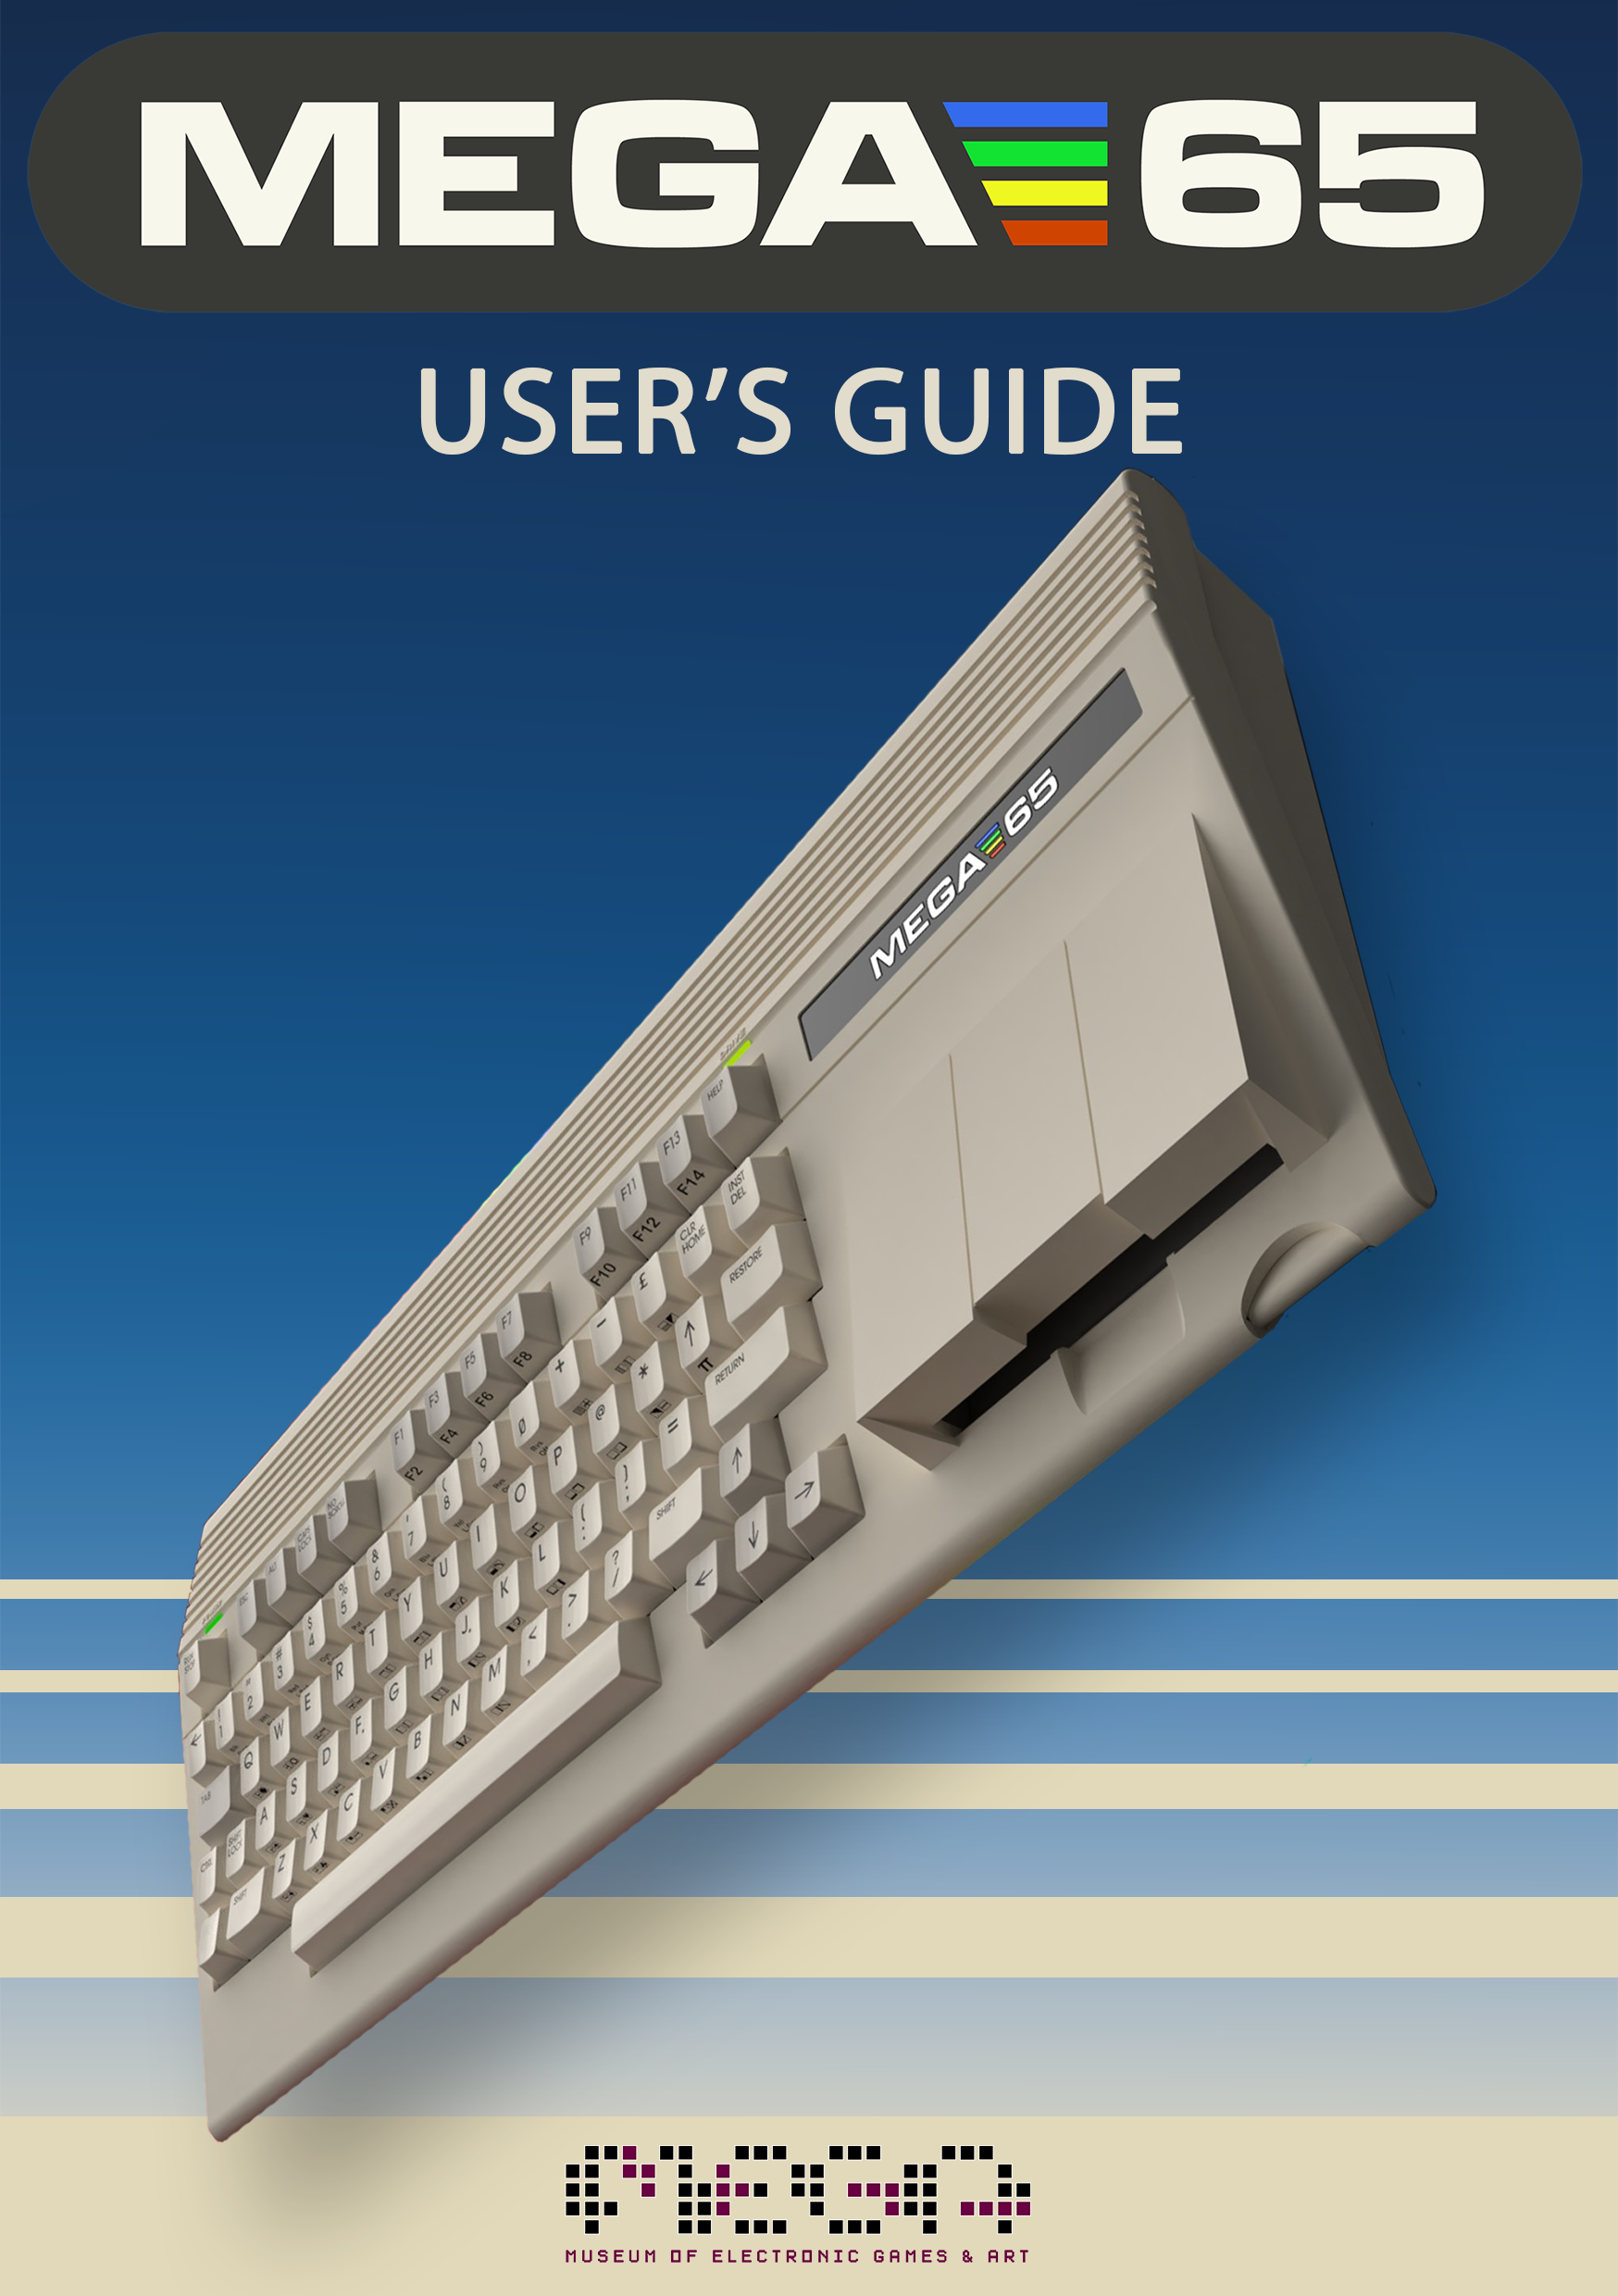
\includegraphics[height=210mm,width=149mm]{frontcover/manual_title}};
\end{tikzpicture}

%\newpage
%\pagecolor{white}

%\vspace*{-2cm}\chapter*{MEGA65 TEAM}
\newpage
{\huge MEGA65 TEAM}\vspace{1cm}

\setlength{\tabcolsep}{1mm}
\begin{tabular}{ll}

{\large\bf Dr. Paul Gardner-Stephen}    & {\large\bf Detlef Hastik} \\
\textit{(highlander)}                   & \textit{(deft)} \\
Founder                                 & Co-Founder \\
Software and Virtual Hardware Architect & General Manager \\
Spokesman and Lead Scientist            & Marketing \& Sales \\
& \\
{\large\bf Martin Streit}               & {\large\bf Anton Schneider-Michallek} \\
 \textit{(seriously)}                   & \textit{(adtbm)} \\
Video and Photo Production              & Hardware Pool Management \\
Tax and Organization                    & Soft-, Hard- and V-Hardware Testing \\
Social Media                            & Forum Administration \\
& \\
{\large\bf Falk Rehwagen}               & {\large\bf Antti Lukats} \\
 \textit{(bluewaysw)}                   & \textit{(antti-brain)} \\
Jenkins Build Automation                & Host Hardware Design and Production \\
GEOS, Hardware Quality Management       & \\
& \\
{\large\bf Dieter Penner}               & {\large\bf Dr. Edilbert Kirk} \\
 \textit{(doubleflash)}                 & \textit{(Bit Shifter)} \\
Host Hardware Review and Testing        & Manual and Tools \\
File Hosting                            & ROM Enhancements \\
& \\
{\large\bf Gábor Lénárt}                & {\large\bf Mirko H.} \\
 \textit{(LGB)}                         & \textit{(sy2002)} \\
Emulator                                & Additional Hardware and Platforms \\
& \\
{\large\bf Farai Aschwanden}            & {\large\bf Thomas Hertzler} \\
 \textit{(Tayger)}                      & \textit{(grumpyninja)} \\
File Base, Tools                        & USA Spokesman \\
Financial Advisory                      & Artist Relations \\
& \\
{\large\bf Andrew Owen}                 & {\large\bf Daniel England} \\
 \textit{(Cheveron)}                    & \textit{(Mew Pokémon)} \\
Keyboard Advisory, Sinclair Support     & Additional Code and Tools \\
& \\
{\large\bf Roman Standzikowski}         & {\large\bf Hernán Di Pietro} \\
 \textit{(FeralChild)}                  & \textit{(indiocolifa)} \\
Open ROMs                               & Additional Emulation \\
\end{tabular}


\chapter*{Reporting Errors and Omissions}

This book is a work-in-progress produced by and for the MEGA65 community.
The version of this edition is:

\input{gitinfo}

We want this book to be the best that it possibly can. So if you see any errors,
find anything that is missing, or would like more information,
please report them using the MEGA65 User's Guide issue tracker:

\url{https://github.com/mega65/mega65-user-guide/issues}

You can also check there to see if anyone else has reported a similar problem,
while you wait for this book to be updated.

Finally, you can always download the latest version of this book from:

\url{https://github.com/mega65/mega65-user-guide}




% paper title
% Titles are generally capitalised except for words such as a, an, and, as,
% at, but, by, for, in, nor, of, on, or, the, to and up, which are usually
% not capitalised unless they are the first or last word of the title.
% Linebreaks \\ can be used within to get better formatting as desired.
% Do not put math or special symbols in the title.

\cleardoublepage

\pagenumbering{roman}

  \begin{titlepage}
    \pagecolor{blue}
     \begin{center}
       {
         \large
         % Put a nice amount of vertical space before the title
         \vspace*{2cm}
               {\Huge\textcolor{white}{\bf{MEGA65 BASIC 10 REFERENCE}}}\\
             \vspace{\fill}
                    {\textcolor{white}
                    {Published by \\ the MEGA Museum of Electronic Games \& Art e.V., Germany.}}
       }
     \end{center}
   \end{titlepage}

% Then the copyright notice page
  \pagecolor{white}\textcolor{black}
  \vfill
  WORK IN PROGRESS

  \index{copyright}Copyright \copyright 2019 -- 2021 by Paul Gardner-Stephen,
  the the MEGA Museum of Electronic Games \& Art e.V.
  and contributors.

  This reference guide is made available under the GNU Free Documentation
  License v1.3, or later, if desired. This means that you are free to
  modify, reproduce and redistribute this user guide, subject to
  certain conditions. The full text of the GNU Free Documentation
  License v1.3 can be found at
  \url{https://www.gnu.org/licenses/fdl-1.3.en.html}.

  Implicit in this copyright license, is the permission to duplicate
  and/or redistribute this document in whole or in part for use in
  education environments. We want to support the education of future
  generations, so if you have any worries or concerns, please contact us.

   \par\today

\newpagestyle{onlynumber}{\setfoot[][{\bf\small\thepage}][]
                                  {} {\bf\small\thepage} {}}
\pagestyle{onlynumber}
\pagecolor{white}

\tableofcontents

%% XXX - big numbers are not in bold, because latex gets confused
\newcommand*{\justifyheading}{\raggedleft}
\definecolor{headingblue}{rgb}{0.5,0.5,1}

% \titleformat{command}[shape]
%   {format}
%   {label}
%   {sep}
%   {before}
%   [after]

% ***************
% PART title page
% ***************

\titleclass{\part}{top}
\titleformat{\part}[display]
   {\thispagestyle{empty}\pagecolor{blue}\normalfont\huge\bfseries\justifyheading}
   {\textcolor{white}{\fontsize{50}{65}\selectfont\bf{PART}\quad{\fontsize{100}{130}\selectfont \bf{\serifed\thepart}}}}
   {20pt}
   {\Huge\textcolor{white}}
   [\newpage\pagecolor{white}\textcolor{black}]

% ******************
% CHAPTER title page
% ******************

\titleformat{\chapter}[display]
   {\thispagestyle{empty}\pagecolor{blue}\normalfont\huge\bfseries\justifyheading}
   {\textcolor{white}{\MakeUppercase{\chaptertitlename}\quad{\fontsize{100}{130}\selectfont \bf\thechapter}}}
   {20pt}
   {\Huge\textcolor{white}}
   [{\chapmtoc\insertminitoc}\newpage\pagecolor{white}\textcolor{black}\cleardoublepage]

% ******************
% SECTION title page
% ******************

\titleformat{\section}[display]
   {\raggedright}
   {\thesection}
   {20pt}
   {\huge\bf\color{headingblue}\uppercase}
   [\color{black}]

\chapter{Introduction}

Congratulations on your purchase of one of the most long-awaited computers in the history of computing. The MEGA65 is a community designed computer, based on the never-released Commodore{\textregistered} 65\footnote{Commodore is a trademark of C= Holdings} computer; a computer designed in 1989 and intended for public release in 1990. Decades have passed, and the MEGA 65 invokes an earlier time when computers were simple and friendly. They were not only simple to operate and understand how they work, but friendly and approachable for new users.

These 1980s computers inspired an entire generation of professionals to choose the exciting and rewarding technology careers they have today. Just imagine the joy of these individuals as they learned they could use their new computer to solve problems, write a letter, prepare taxes, invent new things, or even discover how the universe works. We want to recreate that level of excitement not found in modern computing, so we made the {\bf MEGA65}.

The MEGA65 team believes that owning a computer is like owning a home; you don't just use a home; you change things big and small to make it your own custom living space. After a while, when you settle in, you may decide to renovate or expand your home to make it more comfortable or provide more utility. Think of the MEGA65 as a "computing home."

This guide will teach you how to do more than just hang pictures on a wall, it will ask you to build your dream home. While you read this user's guide, you will learn how to operate the MEGA65, code programs, add additional software, and extend hardware capabilities. What won't be immediately obvious is that along the journey, you will also learn about the history of computing as you explore Commodore BASIC version 10 and operating system commands.

Computer graphics and music make computing more fun; and we designed the MEGA65 for fun! In this user's guide, you will learn to code using the MEGA65's built-in {\bf graphics} and {\bf sound} capabilities. But you don't need to be a coder to have fun with the MEGA65. Because the MEGA65 includes a complete Commodore{\textregistered} 64{\texttrademark}\footnote{Commodore 64 is a trademark of C= Holdings, }, it can also run thousands of games, utilities, and business software from the past and new programs being written today by Commodore enthusiasts. Excitement for the MEGA65 will grow as we discover what programmers as they learn about the power and features of this modern Commodore computer recreation. Together, we will create a whole new "home-brew" community to do things that even we didn't think were possible when creating the MEGA65.

We welcome you on this journey! Thank you for becoming a part of the {\bf MEGA65}community of  users, coders, and enthusiasts! Get involved, learn more about your MEGA65, and join us online at:

% I thought a call to action to join the community would be good to add early on. Where will the final online community call home?


\cleardoublepage
\pagenumbering{arabic}

  \def\drivedefinition{
{\bf drive} drive \# in dual drive disk units. \\
The drive \# defaults to {\bf 0} and can be omitted on single drive units
such as the 1541, 1571, or 1581.
}

\def\unitdefinition{
{\bf unit} device number on the IEC bus.
Typically in the range from 8 to 11 for disk units.
If a variable is used, it must be placed in brackets.
The unit \# defaults to {\bf 8}.
}

\def\filenamedefinition{
{\bf filename} is either a quoted string, e.g. {\bf "data"} or
a string expression in brackets, e.g. {\bf (FI\$)}.
}

  \input{appendix-basic10-indexed}
  \input{appendix-basicabbreviations}
  \input{appendix-screencodes}
  \chapter{Special Keyboard Controls and Sequences}


\section{PETSCII Codes and CHR\$}

\label{appendix:asciicodes}

You can use the \screentext{PRINT CHR\$(X)} statement to print a character.
Below is the full table of PETSCII codes you can print by index.  For example, by
using index 65 from the table below as: \screentext{PRINT CHR\$(65)} you will
print the letter \screentext{A}.

You can also do the reverse with the ASC statement.  For example:
\screentext{PRINT ASC("A")} will output \screentext{65}, which matches with the
code in the table.

Note: Function key (F1-F14 + HELP) values in this table are not intended to be printed via CHR\$(), but rather to allow function-key input to be assessed in BASIC programs via the GET / GETKEY commands.

\begin{adjustwidth}{}{-2cm}
\begin{multicols}{4}
\begin{description}[align=left,labelwidth=0.2cm]
    \item [0]
    \item [1]
    \item [2]   \small{UNDERLINE ON}
    \item [3]
    \item [4]
    \item [5]   \small{WHITE}
    \item [6]
    \item [7]   \small{BELL}
    \item [8]
    \item [9]   \megakey{TAB}
    \item [10]  \small{LINEFEED}
%   \item [11]  \footnotesize{DISABLE \specialkey{SHIFT}\megasymbolkey}
    \item [11]  DISABLE \\ \specialkey{SHIFT}\megasymbolkey
%   \item [12]  \footnotesize{ENABLE \specialkey{SHIFT}\megasymbolkey}
    \item [12]  ENABLE \\ \specialkey{SHIFT}\megasymbolkey
    \item [13]  \megakey{RETURN}
    \item [14]  \small{LOWER CASE}
    \item [15]  \small{BLINK/FLASH ON}
    \item [16]  F9
    \item [17]  \megakey{$\downarrow$}
    \item [18]  \specialkey{RVS ON}
    \item [19]  \specialkey{CLR HOME}
    \item [20]  \specialkey{INST DEL}
    \item [21]  F10 / BACK WORD
    \item [22]  F11
    \item [23]  F12 / NEXT WORD
    \item [24]  SET/CLEAR TAB
    \item [25]  F13
    \item [26]  F14 / BACK TAB
    \item [27]  \small{ESCAPE}
    \item [28]  \small{RED}
    \item [29]  \megakey{$\rightarrow$}
    \item [30]  \small{GREEN}
    \item [31]  \small{BLUE}
    \item [32]  \megakey{SPACE}
    \item [33]  !
    \item [34]  "
    \item [35]  \#
    \item [36]  \$
    \item [37]  \%
    \item [38]  \&
    \item [39]  '
    \item [40]  (
    \item [41]  )
    \item [42]  *
    \item [43]  +
    \item [44]  ,
    \item [45]  -
    \item [46]  .
    \item [47]  /
    \item [48]  0
    \item [49]  1
    \item [50]  2
    \item [51]  3
    \item [52]  4
    \item [53]  5
    \item [54]  6
    \item [55]  7
    \item [56]  8
    \item [57]  9
    \item [58]  :
    \item [59]  ;
    \item [60]  <
    \item [61]  =
    \item [62]  >
    \item [63]  ?
    \item [64]  @
    \item [65]  A
    \item [66]  B
    \item [67]  C
    \item [68]  D
    \item [69]  E
    \item [70]  F
    \item [71]  G
    \item [72]  H
    \item [73]  I
    \item [74]  J
    \item [75]  K
    \item [76]  L
    \item [77]  M
    \item [78]  N
    \item [79]  O
    \item [80]  P
    \item [81]  Q
    \item [82]  R
    \item [83]  S
    \item [84]  T
    \item [85]  U
    \item [86]  V
    \item [87]  W
    \item [88]  X
    \item [89]  Y
    \item [90]  Z
    \item [91]  [
    \item [92]  \pounds
    \item [93]  ]
    \item [94]  $\uparrow$
    \item [95]  $\leftarrow$
    \item [96]  \graphicsymbol{C}
    \item [97]  \graphicsymbol{A}
    \item [98]  \graphicsymbol{B}
    \item [99]  \graphicsymbol{C}
    \item [100] \graphicsymbol{D}
    \item [101] \graphicsymbol{E}
    \item [102] \graphicsymbol{F}
    \item [103] \graphicsymbol{G}
    \item [104] \graphicsymbol{H}
    \item [105] \graphicsymbol{I}
    \item [106] \graphicsymbol{J}
    \item [107] \graphicsymbol{K}
    \item [108] \graphicsymbol{L}
    \item [109] \graphicsymbol{M}
    \item [110] \graphicsymbol{N}
    \item [111] \graphicsymbol{O}
    \item [112] \graphicsymbol{P}
    \item [113] \graphicsymbol{Q}
    \item [114] \graphicsymbol{R}
    \item [115] \graphicsymbol{S}
    \item [116] \graphicsymbol{T}
    \item [117] \graphicsymbol{U}
    \item [118] \graphicsymbol{V}
    \item [119] \graphicsymbol{W}
    \item [120] \graphicsymbol{X}
    \item [121] \graphicsymbol{Y}
    \item [122] \graphicsymbol{Z}
    \item [123] \graphicsymbol{+}
    \item [124] \graphicsymbol{-}
    \item [125] \graphicsymbol{B}
    \item [126] \graphicsymbol{\textbackslash}
    \item [127] \graphicsymbol{]}
    \item [128]
    \item [129] \small{ORANGE}
    \item [130] \small{UNDERLINE OFF}
    \item [131]
    \item [132] HELP
    \item [133] F1
    \item [134] F3
    \item [135] F5
    \item [136] F7
    \item [137] F2
    \item [138] F4
    \item [139] F6
    \item [140] F8
    \item [141] \specialkey{SHIFT}\megakey{RETURN}
    \item [142] \small{UPPERCASE}
    \item [143] \small{BLINK/FLASH OFF}
    \item [144] \small{BLACK}
    \item [145] \megakey{$\uparrow$}
    \item [146] \specialkey{RVS OFF}
    \item [147] \specialkey{SHIFT}\specialkey{CLR HOME}
    \item [148] \specialkey{SHIFT}\specialkey{INST DEL}
    \item [149] \small{BROWN}
    \item [150] \small{LT. RED}
    \item [151] \small{DK. GRAY}
    \item [152] \small{GRAY}
    \item [153] \small{LT. GREEN}
    \item [154] \small{LT. BLUE}
    \item [155] \small{LT. GRAY}
    \item [156] \small{PURPLE}
    \item [157] \megakey{$\leftarrow$}
    \item [158] \small{YELLOW}
    \item [159] \small{CYAN}
    \item [160] \megakey{SPACE}
    \item [161] \graphicsymbol{k}
    \item [162] \graphicsymbol{i}
    \item [163] \graphicsymbol{t}
    \item [164] \graphicsymbol{[}
    \item [165] \graphicsymbol{g}
    \item [166] \graphicsymbol{=}
    \item [167] \graphicsymbol{m}
    \item [168] \graphicsymbol{/}
    \item [169] \graphicsymbol{?}
    \item [170] \graphicsymbol{v}
    \item [171] \graphicsymbol{q}
    \item [172] \graphicsymbol{d}
    \item [173] \graphicsymbol{z}
    \item [174] \graphicsymbol{s}
    \item [175] \graphicsymbol{n}
    \item [176] \graphicsymbol{a}
    \item [177] \graphicsymbol{e}
    \item [178] \graphicsymbol{r}
    \item [179] \graphicsymbol{w}
    \item [180] \graphicsymbol{h}
    \item [181] \graphicsymbol{j}
    \item [182] \graphicsymbol{l}
    \item [183] \graphicsymbol{y}
    \item [184] \graphicsymbol{u}
    \item [185] \graphicsymbol{p}
    \item [186] \graphicsymbol{\{}
    \item [187] \graphicsymbol{f}
    \item [188] \graphicsymbol{c}
    \item [189] \graphicsymbol{x}
    \item [190] \graphicsymbol{v}
    \item [191] \graphicsymbol{b}
\end{description}
\end{multicols}
\end{adjustwidth}
NOTE: Codes for 192 to 223 are the equal to 96-127. Codes 224 to 254 equal to 160-190 and code 255 equal to 126.


\section{Control codes}
\label{appendix:controlcodes}

\begin{center}
\setlength{\def\arraystretch{1.5}\tabcolsep}{6pt}
\begin{longtable}{c|L{5.5cm}}
	\textbf{Keyboard Control} & \textbf{Function}\\
   \hhline{==}
	\endhead

  \multicolumn{2}{l}{\textbf{Colours}} \\
  \hhline{==}
\megakey{CTRL} + \megakey{1} to \megakey{8} &
Choose from the first range of colours.\\
\hline
\megasymbolkey + \megakey{1} to \megakey{8} &
Choose from the second range of colours.\\
\hline
\megakey{CTRL} + \megakey{E} &
Restores the colour of the cursor back to the default white.\\
  \hhline{==}
  \multicolumn{2}{l}{\textbf{Tabs}} \\
  \hhline{==}
\megakey{CTRL} + \megakey{Z} &
Tabs the cursor to the left. When there are no more tab positions, the cursor will remain at the start of the line.\\
\hline
\megakey{CTRL} + \megakey{I} &
Tabs the cursor to the right. When there are no more tab positions, the cursor will remain at the end of the line.\\
\hline
\megakey{CTRL} + \megakey{X} &
Sets or clears the current screen column as a tab position.
 Use \megakey{CTRL} + \megakey{I} and \megakey{Z} to jump to all positions set with \megakey{X}.\\
  \hhline{==}
  \multicolumn{2}{l}{\textbf{Movement}} \\
  \hhline{==}
\megakey{CTRL} + \megakey{Q} &
Moves the cursor down one line at a time. This is the same function produced by the \megakey{$\downarrow$} key.\\
\hline
\megakey{CTRL} + \megakey{J} &
Moves the cursor down a row. If you are on a long line of BASIC code that has extended to two lines, then the cursor will move down two positions to point to the next line.\\
\hline
\megakey{CTRL} + \megakey{]} &
The same function as \megakey{$\rightarrow$}.\\
\hline
\megakey{CTRL} + \megakey{T} &
Backspace the character immediately to the left and to shift all rightmost characters one position to the left. This is the same function as the \specialkey{INST DEL} key.\\
\hline
\megakey{CTRL} + \megakey{M} &
Performs a carriage return, the same function as the \megakey{Return} key.\\

  \hhline{==}
  \multicolumn{2}{l}{\textbf{Word movement}} \\
  \hhline{==}

\megakey{CTRL} + \megakey{U} &
Moves cursor back to the start of the previous word, or unbroken string of characters. If there are no characters between the current cursor position and the start of the line, the cursor will move to the first column of the current line.\\
\hline
\megakey{CTRL} + \megakey{W} &
Advances cursor forward to the start of the next word, or unbroken string of characters. If there are no characters between the current cursor position and the end of the line, the cursor will move to the first column of the next line.\\

  \hhline{==}
  \multicolumn{2}{l}{\textbf{Scrolling}} \\
  \hhline{==}

\megakey{CTRL} + \megakey{P} &
Scroll BASIC listing down one line, equivalent to \megakey{F9} key.\\
\hline
\megakey{CTRL} + \megakey{V} &
Scroll BASIC listing up one line, equivalent to \megakey{F11} key.\\
\hline
\megakey{CTRL} + \megakey{S} &
Equivalent to \specialkey{NO\\SCROLL} key.\\

  \hhline{==}
  \multicolumn{2}{l}{\textbf{Formatting}} \\
  \hhline{==}

\megakey{CTRL} + \megakey{B} &
Turns on underline text mode. Turn off underline mode by pressing \megakey{ESC} then \megakey{O}.\\
\hline
\megakey{CTRL} + \megakey{O} &
Turns on flashing text mode. Turn off flashing mode by pressing \megakey{ESC} then \megakey{O}.\\
\hline

  \hhline{==}
  \multicolumn{2}{l}{\textbf{Casing}} \\
  \hhline{==}

\megakey{CTRL} + \megakey{N} &
Changes the text case mode from uppercase to lowercase.\\
\hline
\megakey{CTRL} + \megakey{K} &
Locks the uppercase/lowercase mode switch usually performed with \megasymbolkey and \megakey{Shift} keys.\\
\hline
\megakey{CTRL} + \megakey{L} &
Enables the uppercase/lowercase mode switch that is performed with the \megasymbolkey and \megakey{Shift} keys.\\

  \hhline{==}
  \multicolumn{2}{l}{\textbf{Miscellaneous}} \\
  \hhline{==}

\megakey{CTRL} + \megakey{G} &
Produces a bell tone.\\
\hline
\megakey{CTRL} + \megakey{[} &
Equivalent to pressing the \megakey{ESC} key.\\
\hline
\megakey{CTRL} + \megakey{*} &
Enters the Matrix Mode Debugger.\\
\hline

\end{longtable}
\end{center}

\newpage

\section{Shifted codes}
\label{appendix:shiftedcodes}

\begin{center}
\setlength{\def\arraystretch{1.5}\tabcolsep}{6pt}
\begin{longtable}{c|L{5.5cm}}
	\textbf{Keyboard Control} & \textbf{Function}\\
  \hhline{==}
	\endhead

\megakey{Shift} + \specialkey{INST DEL} &
Insert a character in the current cursor position and move all characters to the right by one position.\\
\hline
\megakey{Shift} + \specialkey{HOME} &
Clear home, clear the entire screen and move the cursor to the home position.\\
\hline

\end{longtable}
\end{center}



\section{Escape Sequences}
\label{appendix:escapesequences}

To perform an Escape Sequence, press and release the \megakey{ESC} key. Then press one of the following keys to perform the sequence:

\begin{center}
\setlength{\def\arraystretch{1.5}\tabcolsep}{6pt}
\begin{longtable}{c|L{5.5cm}}
	\textbf{Key} & \textbf{Sequence}\\
  \hhline{==}
	\endhead

  \multicolumn{2}{l}{\textbf{Editor behaviour}} \\
  \hhline{==}
\megakey{ESC} \megakey{X} &
Clears the screen and toggles between 40 and 80 column modes.\\
\hline
\megakey{ESC} \megakey{@} &
Clears the screen starting from the cursor to the end of the screen.\\
\hline
\megakey{ESC} \megakey{O} &
Cancels the quote, reverse, underline and flash modes.\\
  \hhline{==}
  \multicolumn{2}{l}{\textbf{Scrolling}} \\
  \hhline{==}
\hline
\megakey{ESC} \megakey{V} &
Scrolls the entire screen up one line.\\
\hline
\megakey{ESC} \megakey{W} &
Scrolls the entire screen down one line.\\
\hline
\megakey{ESC} \megakey{L} &
Enables scrolling when the cursor down key is pressed at the bottom of the screen.\\
\hline
\megakey{ESC} \megakey{M} &
Disables scrolling. When pressing the cursor down key at the bottom on the screen, the cursor will move to the top of the screen. The cursor is restricted at the top of the screen with the Cursor up key.\\
  \hhline{==}
  \multicolumn{2}{l}{\textbf{Insertion and deletion}} \\
  \hhline{==}
\megakey{ESC} \megakey{I} &
Inserts an empty line in the current cursor position and moves all subsequent lines down one position.\\
\hline
\megakey{ESC} \megakey{D} &
Deletes the current line and moves other lines up one position.\\
\hline
\megakey{ESC} \megakey{P} &
Erases all characters from the cursor to the start of current line.\\
\hline
\megakey{ESC} \megakey{Q} &
Erases all characters from the cursor to the end of current line.\\
  \hhline{==}
  \multicolumn{2}{l}{\textbf{Movement}} \\
  \hhline{==}
\megakey{ESC} \megakey{J} &
Moves the cursor to start of current line.\\
\hline
\megakey{ESC} \megakey{K} &
Move to end of the last non-white-space character on the current line.\\
\hline
\megakey{ESC} $\uparrow$ &
Saves the current cursor position. Use \megakey{ESC} $\leftarrow$ key (next to 1 key) to move back to saved position.\\
\hline
\megakey{ESC} $\leftarrow$ &
Restores the cursor position to the position stored via a prior press of the \megakey{ESC} $\uparrow$ key (next to RESTORE key).\\
  \hhline{==}
  \multicolumn{2}{l}{\textbf{Windowing}} \\
  \hhline{==}
\megakey{ESC} \megakey{T} &
Set top-left window area of the screen at the cursor position. All typed characters and screen activity will be restricted to the area. Also see \megakey{ESC} then \megakey{B}.\\
\hline
\megakey{ESC} \megakey{B} &
Sets the bottom-right window area of the screen at the cursor position. All typed characters and screen activity will be restricted to the area. Also see \megakey{ESC} then \megakey{T}.\\
  \hhline{==}
  \multicolumn{2}{l}{\textbf{Cursor behaviour}} \\
  \hhline{==}
\megakey{ESC} \megakey{A} &
Enables the auto-insert mode. Any keys pressed will insert before other characters.\\
\hline
\megakey{ESC} \megakey{C} &
Disables auto-insert mode, going back to overwrite mode.\\
\hline
\megakey{ESC} \megakey{E} &
Sets the cursor to non-flashing mode.\\
\hline
\megakey{ESC} \megakey{F} &
Sets the cursor to regular flashing mode.\\
  \hhline{==}
  \multicolumn{2}{l}{\textbf{Bell behaviour}} \\
  \hhline{==}
\megakey{ESC} \megakey{G} &
Enables the bell which can be sounded using \megakey{CTRL} and \megakey{G}.\\
\hline
\megakey{ESC} \megakey{H} &
Disable the bell so that pressing \megakey{CTRL} and \megakey{G} will have no effect.\\
  \hhline{==}
  \multicolumn{2}{l}{\textbf{Colours}} \\
  \hhline{==}
\megakey{ESC} \megakey{S} &
Switches the VIC-IV to colour range 16-31. These colours can be accessed with \megakey{CTRL} and keys \megakey{1} to \megakey{8} or \megasymbolkey and keys \megakey{1} to \megakey{8}.\\
\hline
\megakey{ESC} \megakey{U} &
Switches the VIC-IV to colour range 0-15. These colours can be accessed with \megakey{CTRL} and keys \megakey{1} to \megakey{8} or \megasymbolkey and keys \megakey{1} to \megakey{8}.\\
\hline
  \hhline{==}
  \multicolumn{2}{l}{\textbf{Tabs}} \\
  \hhline{==}
\megakey{ESC} \megakey{Y} &
Set the default tab stops (every 8 spaces) for the entire screen.\\
\hline
\megakey{ESC} \megakey{Z} &
Clears all the tab stops. Any tabbing with \megakey{CTRL} and \megakey{I} will move the cursor to the end of the line.\\
\hline
\end{longtable}
\end{center}

  \input{appendix-screenmaps}
  \input{appendix-error-messages}
  \chapter{Supporters \& Donors}

The MEGA65 would not have been possible to create without the generous support
of many organisations and individuals.

We are still compiling these lists, so apologies if we haven't included you yet.  If you
know anyone we have left out, please let us know, so that we can recognise the contribution
of everyone who has made the MEGA65 possible, and into the great retro-computing project
that it has become.

\section{Organisations}

\begin{itemize}
\item {\bf The MEGA Museum of Electronic Games \& Art e.V. Germany} \megakey{Everything}
\item {\bf Trenz Electronik, Germany} \megakey{Motherboard}
\item {\bf Hintsteiner, Austria} \megakey{Case}
\item {\bf GMK, Germany} \megakey{Keyboard}
\end{itemize}

\section{Contributors}

\setlength{\tabcolsep}{1mm}
\begin{tabular}{p{6cm}p{6cm}}

{\large\bf Andreas Liebeskind}     & {\large\bf Dr. Canan Hastik} \\
 \textit{(libi in paradize)}       & \textit{(indica)} \\
CFO MEGA eV                        & Chairwoman MEGA eV \\
& \\
{\large\bf Gurce Isikyildiz}       & {\large\bf Simon Jameson} \\
 \textit{(Gurce)}                  &  \textit{(Shallan)} \\
Tools and enhancements             & Platform Enhancements \\
& \\
{\large\bf Russell Peake}          & {\large\bf Stephan Kleinert} \\
  \textit{(rdpeake)}               & \textit{(ubik)}        \\
Bug Herding                        & Destroyer of BASIC 10     \\
& \\
{\large\bf Alexander Nik Petra}    & {\large\bf Wayne Johnson} \\
 \textit{(n0d)}                    &  \textit{(sausage)} \\
Early Case Design                  & Manual Additions \\
& \\
{\large\bf Ralph Egas}             & {\large\bf Lukas Kleiss} \\
 \textit{(0-limits)}               & \textit{(LAK132)} \\
Business Advisor                   & MegaWAT Presentation Software \\
& \\
{\large\bf Lucas Moss}             & {\large\bf Maurice van Gils }  \\
                                   & \textit{(Maurice)}  \\
MEGAphone PCB Design               & BASIC-65 example programs \\
& \\
{\large\bf Daren Klamer}           \\
 \textit{(Impakt)}                 \\
Manual proof-reading               \\
& \\
\end{tabular}

\newpage
\section{Supporters}

% page 1
\setlength{\tabcolsep}{1mm}
\begin{tabular}{p{4.5cm}p{4.5cm}p{4.5cm}}
@11110110100 & Arne Neumann & Christian Gräfe \\
3c74ce64 & Arne Richard Tyarks & Christian Heffner \\
8-Bit Classics & Axel Klahr & Christian Kersting \\
Aaron Smith & Balaz Ondrej & Christian Streck \\
Achim Mrotzek & Barry Thompson & Christian Wyk \\
Adolf Nefischer & Benjamin Maas & Christoph Haug \\
Adrian Esdaile & Bernard Alaiz & Christoph Huck \\
Adrien Guichard & Bernhard Zorn & Christoph Pross \\
Ahmed Kablaoui & Bieno Marti-Braitmaier & Christopher Christopher \\
Alan Bastian Witkowski & Bigby & Christopher Kalk \\
Alan Field & Bill LaGrue & Christopher Kohlert \\
Alberto Mercuri & Bjoerg Stojalowski & Christopher Nelson \\
Alexander Haering & Björn Johannesson & Christopher Taylor \\
Alexander Kaufmann & Bjørn Melbøe & Christopher Whillock \\
Alexander Niedermeier & Bo Goeran Kvamme & Claudio Piccinini \\
Alexander Soppart & Boerge Noest & Claus Skrepek \\
Alfonso Ardire & Bolko Beutner & Collen Blijenberg \\
Amiga On The Lake & Brett Hallen & Constantine Lignos \\
Andre Kapp & Brian Gajewski & Crnjaninja \\
André Kudra & Brian Green & Daniel Auger \\
André Simeit & Brian Juul Nielsen & Daniel Julien \\
André Wösten & Brian Reiter & Daniel Lobitz \\
Andrea Farolfi & Bryan Pope & Daniel O'Connor \\
Andrea Minutello & Burkhard Franke & Daniel Teicher \\
Andreas Behr & Byron Goodman & Daniel Tootill \\
Andreas Freier & Cameron Roberton (KONG) & Daniel Wedin \\
Andreas Grabski & Carl Angervall & Daniele Benetti \\
Andreas Millinger & Carl Danowski & Daniele Gaetano Capursi \\
Andreas Nopper & Carl Stock & Dariusz Szczesniak \\
Andreas Wendel Manufaktur & Carl Wall & Darrell Westbury \\
Andreas Zschunke & Carlo Pastore & David Asenjo Raposo \\
Andrew Bingham & Carlos Silva & David Dillard \\
Andrew Dixon & Carsten Sørensen & David Gorgon \\
Andrew Mondt & Cenk Miroglu Miroglu & David Norwood \\
Andrzej Hłuchyj & Chang sik Park & David Raulo \\
Andrzej Sawiniec & Charles A. Hutchins Jr. & David Ross \\
Andrzej Śliwa & Chris Guthrey & de voughn accooe \\
Anthony W. Leal & Chris Hooper & Dean Scully \\
Arkadiusz Bronowicki & Chris Stringer & Dennis Jeschke \\
Arkadiusz Kwasny & Christian Boettcher & Dennis Schaffers \\
Arnaud Léandre & Christian Eick & Dennis Schierholz \\
Arne Drews & Christian Gleinser & Dennis Schneck \\
\end{tabular}
% page 2
\newpage
\setlength{\tabcolsep}{1mm}
\begin{tabular}{p{4.5cm}p{4.5cm}p{4.5cm}}
denti & Frank Hempel & Henning Harperath \\
Dick van Ginkel & Frank Koschel & Henri Parfait \\
Diego Barzon & Frank Linhares & Henrik Kühn \\
Dierk Schneider & Frank Wolf & Holger Burmester \\
Dietmar Krueger & FranticFreddie & Holger Sturk \\
Dietmar Schinnerl & Fredrik Ramsberg & Howard Knibbs \\
Dirk Becker & Fridun Nazaradeh & Hubert de Hollain \\
Dirk Wouters & Friedel Kropp & Huberto Kusters \\
Domingo Fivoli & Garrick West & Hugo Maria Gerardus v.d. Aa \\
DonChaos & Gary Lake-Schaal & Humberto Castaneda \\
Donn Lasher & Gary Pearson & Ian Cross \\
Douglas Johnson & Gavin Jones & IDE64 Staff \\
Dr. Leopold Winter & Geir Sigmund Straume & Igor Ianov \\
Dusan Sobotka & Gerd Mitlaender & Immo Beutler \\
Earl Woodman & Giampietro Albiero & Ingo Keck \\
Ed Reilly & Giancarlo Valente & Insanely Interested Publishing \\
Edoardo Auteri & Gianluca Girelli & IT-Dienstleistungen Obsieger \\
Eduardo Gallardo & Giovanni Medina & Ivan Elwood \\
Eduardo Luis Arana & Glen Fraser & Jaap HUIJSMAN \\
Eirik Juliussen Olsen & Glen R Perye III & Jace Courville \\
Emilio Monelli & Glenn Main & Jack Wattenhofer \\
EP Technical Services & Gordon Rimac & Jakob Schönpflug \\
Epic Sound & GRANT BYERS & Jakub Tyszko \\
Erasmus Kuhlmann & Grant Louth & James Hart \\
ergoGnomik & Gregor Bubek & James McClanahan \\
Eric Hildebrandt & Gregor Gramlich & James Sutcliffe \\
Eric Hill & Guido Ling & Jan Bitruff \\
Eric Jutrzenka & Guido von Gösseln & Jan Hildebrandt \\
Erwin Reichel & Guillaume Serge & Jan Iemhoff \\
Espen Skog & Gunnar Hemmerling & Jan Kösters \\
Evangelos Mpouras & Günter Hummel & Jan Peter Borsje \\
Ewan Curtis & Guy Simmons & Jan Schulze \\
Fabio Zanicotti & Guybrush Threepwood & Jan Stoltenberg-Lerche \\
Fabrizio Di Dio & Hakan Blomqvist & Janne Tompuri \\
Fabrizio Lodi & Hans Pronk & Jannis Schulte \\
FARA Gießen GmbH & Hans-Jörg Nett & Jari Loukasmäki \\
FeralChild & Hans-Martin Zedlitz & Jarrod Adams \\
First Choice Auto's & Harald Dosch & Jason Smith \\
Florian Rienhardt & Harri Salokorpi & Javier Gonzalez Gonzalez \\
Forum64. de & Harry Culpan & Jean-Paul Lauque \\
Francesco Baldassarri & Heath Gallimore & Jeffrey van der Schilden \\
Frank Fechner & Heinz Roesner & Jens Schneider \\
Frank Glaush & Heinz Stampfli & Jens-Uwe Wessling \\
Frank Gulasch & Helge Förster & Jesse DiSimone \\
Frank Haaland & Hendrik Fensch & Johan Arneklev \\
\end{tabular}
% page 3
\newpage
\setlength{\tabcolsep}{1mm}
\begin{tabular}{p{4.5cm}p{4.5cm}p{4.5cm}}
Johan Svensson & Kosmas Einbrodt & Marcus Linkert \\
Johannes Fitz & Kurt Klemm & Marek Pernicky \\
John Cook & Lachlan Glaskin & Mario Esposito \\
John Deane & Large bits collider & Mario Fetka \\
John Nagi & Lars Becker & Mario Teschke \\
John Rorland & Lars Berntsson & Mariusz Tymków \\
John Sargeant & Lars Edelmann & Mark Adams \\
John Traeholt & Lars Slivsgaard & Mark Green \\
Jon Sandelin & Lasse Lambrecht & Mark Hucker \\
Jonas Bernemann & Lau Olivier & Mark Leitiger \\
Jonathan Prosise & Lee Chatt & Mark Spezzano \\
Joost Honig & Loan Leray & Mark Watkin \\
Jordi Pakey-Rodriguez & Lorenzo Quadri & Marko Rizvic \\
Jöre Weber & Lorenzo Travagli & Markus Bieler \\
Jörg Jungermann & Lorin Millsap & Markus Bonet \\
Jörg Schaeffer & Lothar James Foss & Markus Dauberschmidt \\
Jörg Weese & Lothar Serra Mari & Markus Fehr \\
Josef Hesse & Luca Papinutti & Markus Fuchs \\
Josef Soucek & Ludek Smetana & Markus Guenther-Hirn \\
Josef Stohwasser & Lukas Burger & Markus Liukka \\
Joseph Gerth & Lutz-Peter Buchholz & Markus Merz \\
Jovan Crnjanin & Luuk Spaetgens & Markus Roesgen \\
Juan Pablo Schisano & Mad Web Skills & Markus Uttenweiler \\
Juan S. Cardona Iguina & MaDCz & Martin Bauhuber \\
JudgeBeeb & Magnus Wiklander & Martin Benke \\
Juliussen Olsen & Maik Diekmann & Martin Gendera \\
Juna Luis Fernandez Garcia & Malte Mundt & Martin Groß \\
Jürgen Endras & Manfred Wittemann & Martin Gutenbrunner \\
Jürgen Herm Stapelberg & Manuel Beckmann & Martin Johansen \\
Jyrki Laurila & Manzano Mérida & Martin Marbach \\
Kai Pernau & Marc "3D-vice" Schmitt & Martin Sonnleitner \\
Kalle Pöyhönen & Marc Bartel & Martin Steffen \\
Karl Lamford & Marc Jensen & Marvin Hardy \\
Karl-Heinz Blum & Marc Schmidt & Massimo Villani \\
Karsten Engstler & Marc Theunissen & Mathias Dellacherie \\
Karsten Westebbe & Marc Tutor & Mathieu Chouinard \\
Keith McComb & Marc Wink & Matthew Adams \\
Kenneth Dyke & Marcel Buchtmann & Matthew Browne \\
Kenneth Joensson & Marcel Kante & Matthew Carnevale \\
Kevin Edwards & Marco Beckers & Matthew Palmer \\
Kevin Thomasson & Marco Cappellari & Matthew Santos \\
Kim Jorgensen & Marco Rivela & Matthias Barthel \\
Kim Rene Jensen & Marco van de Water & Matthias Dolenc \\
Kimmo Hamalainen & Marcus Gerards & Matthias Fischer \\
Konrad Buryło & Marcus Herbert & Matthias Frey \\
\end{tabular}
% page 4
\newpage
\setlength{\tabcolsep}{1mm}
\begin{tabular}{p{4.5cm}p{4.5cm}p{4.5cm}}
Matthias Grandis & Mikko Hämäläinen & Pauline Brasch \\
Matthias Guth & Mikko Suontausta & Paulo Apolonia \\
Matthias Lampe & Mirko Roller & Pete Collin \\
Matthias Meier & Miroslav Karkus & Pete of Retrohax.net \\
Matthias Mueller & Morgan Antonsson & Peter Eliades \\
Matthias Nofer & Moritz & Peter Gries \\
Matthias Schonder & Morten Nielsen & Peter Habura \\
Max Ihlenfeldt & MUBIQUO APPS,SL & Peter Herklotz \\
Meeso Kim & Myles Cameron-Smith & Peter Huyoff \\
Michael Dailly & Neil Moore & Peter Leswell \\
Michael Dötsch & Nelson & Peter Weile \\
Michael Dreßel & neoman & Petri Alvinen \\
Michael Fichtner & Nicholas Melnick & Philip Marien \\
Michael Fong & Nikolaj Brinch Jørgensen & Philip Timmermann \\
Michael Geoffrey Stone & Nils Andreas & Philipp Rudin \\
Michael Gertner & Nils Eilers & Pierre Kressmann \\
Michael Grün & Nils Hammerich & Pieter Labie \\
Michael Habel & Nils77 & Piotr Kmiecik \\
Michael Härtig & Norah Smith & Power-on.at \\
Michael Haynes & Norman King & Przemysław Safonow \\
Michael J Burkett & Normen Zoch & Que Labs \\
Michael Jensen & Olaf Grunert & R Welbourn \\
Michael Jurisch & Ole Eitels & R-Flux \\
Michael Kappelgaard & Oliver Boerner & Rafał Michno \\
Michael Kleinschmidt & Oliver Brüggmann & Rainer Kappler \\
Michael Lorenz & Oliver Graf & Rainer Weninger \\
Michael Mayerhofer & Oliver Smith & Ralf Griewel \\
Michael Nurney & Olivier Bori & Ralf Reinhardt \\
Michael Rasmussen & ONEPSI LLC & Ralf Schenden \\
Michael Richmond & oRdYNe & Ralf Smolarek \\
Michael Sachse & Osaühing Trioflex & Ralf Zenker \\
Michael Sarbak & OSHA-PROS USA & Ralph Bauer \\
Michael Scholz & Padawer & Ralph Wernecke \\
Michael Timm & Patrick Becher & Rédl Károly \\
Michael Traynor & Patrick Bürckstümmer & Reiner Lanowski \\
Michael Whipp & Patrick de Zoete & Remi Veilleux \\
Michal Ursiny & Patrick Toal & Riccardo Bianchi \\
Michele Chiti & Patrick Vogt & Richard Englert \\
Michele Perini & Paul Alexander Warren & Richard Good \\
Michele Porcu & Paul Gerhardt (KONG) & Richard Menedetter \\
Miguel Angel Rodriguez Jodar & Paul Jackson & Richard Sopuch \\
Mikael Lund & Paul Johnson & Rick Reynolds \\
Mike Betz & Paul Massay & Rico Gruninger \\
Mike Kastrantas & Paul Westlake & Rob Dean \\
Mike Pikowski & Paul Woegerer & Robert Bernardo \\
\end{tabular}
% page 5
\newpage
\setlength{\tabcolsep}{1mm}
\begin{tabular}{p{4.5cm}p{4.5cm}p{4.5cm}}
Robert Eaglestone & Stefan Haberl & Thomas Schilling \\
Robert Grasböck & Stefan Kramperth & Thomas Tahsin-Bey \\
Robert Miles & Stefan Richter & Thomas Walter \\
Robert Schwan & Stefan Schultze & Thomas Wirtzmann \\
Robert Shively & Stefan Sonnek & Thorsten Knoll \\
Robert Tangmar & Stefan Theil & Thorsten Nolte \\
Robert Trangmar & Stefan Vrampe & Tim Krome \\
Rodney Xerri & Stefano Canali & Tim Waite \\
Roger Olsen & Stefano Mozzi & Timo Weirich \\
Roger Pugh & Steffen Reiersen & Timothy Blanks \\
Roland Attila Kett & Stephan Bielmann & Timothy Henson \\
Roland Evers & Stephen Jones & Timothy Prater \\
Roland Schatz & Steve Gray & Tobias Butter \\
Rolf Hass & Steve Kurlin & Tobias Heim \\
Ronald Cooper & Steve Lemieux & Tobias Köck \\
Ronald Hunn & Steven Combs & Tobias Lüthi \\
Ronny Hamida & Stewart Dunn & Tommi Vasarainen \\
Ronny Preiß & Stuart Marsh & Toni Ammer \\
Roy van Zundert & Sven Neumann & Tore Olsen \\
Rüdiger Wohlfromm & Sven Stache & Torleif Strand \\
Ruediger Schlenter & Sven Sternberger & Torsten Schröder \\
Rutger WIllemsen & Sven Wiegand & Tuan Nguyen \\
Sampo Peltonen & Szabolcs Bence & Uffe Jakobsen \\
Sarmad Gilani & Tantrumedia Limited & Ulrich Hintermeier \\
SAS74 & Techvana Operations Ltd. & Ulrich Nieland \\
Scott Halman & Teddy Turmeaux & Ulrik Kruse \\
Scott Hollier & Teemu Korvenpää & Ursula Förstle \\
Scott Robison & The Games Foundation & Uwe Boschanski \\
Sebastian Baranski & Thierry Supplisson & Vedran Vrbanc \\
Sebastian Bölling & Thieu-Duy Thai & Verm Project \\
Sebastian Felzmann & Thomas Bierschenk & Wayne Sander \\
Sebastian Lipp & Thomas Edmister & Wayne Steele \\
Sebastian Rakel & Thomas Frauenknecht & Who Knows \\
Şemseddin Moldibi & Thomas Gitzen & Winfried Falkenhahn \\
Seth Morabito & Thomas Gruber & Wolfgang Becker \\
Shawn McKee & Thomas Haidler & Wolfgang Stabla \\
Siegfried Hartmann & Thomas Jager & Worblehat \\
Sigurbjorn Larusson & Thomas Karlsen & www.patop69.net \\
Sigurdur Finnsson & Thomas Laskowski & Yan B \\
Simon Lawrence & Thomas Marschall & Zoltan Markus \\
Simon Wolf & Thomas Niemann & Zytex Online Store \\
spreen.digital & Thomas Scheelen &  \\
\end{tabular}



\nocite{*}
\bibliographystyle{IEEEtran}
\bibliography{references}

\printindex


\end{document}


